\documentclass[notitlepage,12pt]{jedm}

\usepackage[table]{xcolor}
\usepackage{url}
\usepackage{hyperref}
\usepackage{graphicx}
\graphicspath{{figures/}}
\usepackage{amsmath,amssymb,amsfonts}
\usepackage{algorithmic}
\usepackage{algorithm}
\usepackage{array}
\usepackage{booktabs}
\hypersetup{
  colorlinks = true,
  urlcolor   = blue,
  linkcolor  = blue,
  citecolor  = blue
}

\begin{document}

\title{Personalizing Open-Domain Video Curricula: A Hybrid Closed-Loop Framework Combining Contextual Bandits, Difficulty-Conditioned BKT, and Interaction Telemetry}
\date{}

\author{{\large Kavya Aggarwal}\\Department of Computer Science and Engineering\\GITAM (Deemed to be University), Hyderabad, Telangana, India\\kaggarwa@gitam.in}

\maketitle

\begin{abstract}
Video-based instruction dominates modern Massive Open Online Courses (MOOCs), but passive viewing suffers from rapid cognitive decay and a lack of individualized pacing. Retrieval practice (formative in-video checkpoints) is a well-established remedy, but deploying it at scale requires automated, factually-grounded question generation, since manually authoring assessments for arbitrary lecture content does not scale and ungrounded large language models (LLMs) risk hallucination. We present CogniLoop, a closed-loop system combining (1) a Retrieval-Augmented Generation (RAG) pipeline for transcript-grounded assessment generation, addressing the content-authoring bottleneck directly; (2) a Difficulty-Conditioned Bayesian Knowledge Tracing (DC-BKT) engine for per-learner mastery tracking; (3) a Thompson Sampling contextual bandit for difficulty routing; and (4) $K$-Means interaction-telemetry clustering ($K=3$, silhouette score $0.64$). We evaluate each component individually rather than assuming architectural completeness implies empirical benefit. In an algorithmic simulation across $N=60$ learner profiles, CogniLoop showed a statistically significant increase in Simulated Normalized Learning Gain (NLG) over static video viewing ($\Delta\text{NLG}=+0.541$, Welch's $t(45.4)=3.768$, $p=4.73\times10^{-4}$, Cohen's $d=0.973$, Mann-Whitney $U=709.5$). A component-isolation ablation attributes this gain to checkpoint frequency, not routing: holding checkpoint rate constant, bandit-routed selection underperformed a fixed-medium baseline ($-0.069$ NLG), corroborated by an independent logistic regression on step-level data. A multi-parameter sensitivity sweep further shows the effect is not robust to small perturbations of the checkpoint-rate parameter (only 1 of 8 configurations remained significant). Every statistic reported, including negative and fragility findings, is independently reproducible from committed, seeded source code. We frame this as Phase 1 of a multi-phase research agenda: the RAG-grounded content-generation architecture and the checkpoint-frequency effect are validated contributions, while difficulty-routing tuning is scoped as concrete future work preceding live classroom trials. The code and all reproducibility scripts are available at https://github.com/OmegaKavya/CogniLoop.\\

{\parindent0pt
\textbf{Keywords:} adaptive learning, Bayesian knowledge tracing, contextual bandits, retrieval-augmented generation, reproducibility
}
\end{abstract}

\section{Introduction}
Video-based educational repositories (e.g., Coursera, edX, YouTube Edu) have democratized access to university-level computing curricula. Millions of learners engage daily with asynchronous video lectures. Despite this reach, empirical research in cognitive psychology demonstrates that passive video consumption frequently engenders an illusion of competence \cite{dunlosky2013improving,karpicke2008critical}. Without deliberate retrieval practice, learners experience rapid memory decay characterized by Ebbinghaus forgetting curves.

To counteract passive decay, Intelligent Tutoring Systems (ITS) insert formative assessments, cognitive scaffolds, and adaptive remedial loops into the learning pathway \cite{koedinger1997intelligent,bloom19842,vanlehn2006behavior}. Traditional rule-based and graph-based ITS (such as Cognitive Tutors or ASSISTments) have established the pedagogical superiority of individualized instruction. However, scaling traditional ITS to thousands of diverse open-domain lecture videos is severely limited by the Content-Authoring Bottleneck: manually formulating domain models, misconception-specific distractors, hints, and skill graphs requires hundreds of hours of expert intervention per instructional hour.

Recently, generative Large Language Models (LLMs) have emerged as powerful candidates for automated assessment synthesis \cite{scarlatos2024distractor,dan2023educhat,pardos2023chatgpt}. Nevertheless, deploying naive LLM prompting within tutoring systems introduces two substantial technical challenges: (1) Factual Drift and Hallucination -- unconstrained LLMs frequently introduce extraneous concepts, incorrect distractor logic, or syllabus misalignment when generating questions without explicit context grounding \cite{gao2023retrieval,niu2024reducing}; and (2) Absence of Latent Cognitive Modeling -- standalone conversational LLM interfaces lack explicit probabilistic representations of learner knowledge states over time, rendering them incapable of mathematically optimizing learning trajectories or pacing \cite{piech2015deep,pelanek2017bayesian,doroudi2019where}.

\subsection{Why a Multi-Component Architecture}
Before detailing our contributions, we address directly why CogniLoop integrates four subsystems rather than deploying retrieval practice alone. This paper's own Phase 1 findings (Section~5) show that active-retrieval checkpointing accounts for the measured simulated learning-gain advantage, while difficulty-routing does not yet show a measured benefit in isolation. This is not evidence that the architecture is unnecessary: RAG grounding and DC-BKT exist to solve a \emph{different} problem than learning-gain optimization, namely the content-authoring bottleneck and factual-drift risk inherent to open-domain LLM-based question generation, which retrieval practice alone does not address, since manually authoring misconception-aware questions for arbitrary video content does not scale. Interaction telemetry clustering exists to support engagement monitoring and cold-start context, independent of the difficulty-routing question. We therefore present CogniLoop as an integrated \emph{systems} contribution whose components address distinct engineering problems (automated, grounded content generation at scale; fault-tolerant deployment; cognitive state tracking; engagement monitoring), evaluated individually wherever possible (Section~5), rather than as a monolithic claim that every component improves learning gain. Where a component's contribution to learning gain is not yet empirically supported, we report that directly instead of implying it.

\subsection{Our Contributions}
To resolve the dichotomy between static handcrafted ITS and ungrounded generative interfaces, we introduce CogniLoop, an integrated, closed-loop adaptive learning system.\footnote{Source code and implementation: \url{https://github.com/OmegaKavya/CogniLoop}} The contributions of this work are fourfold:
\begin{itemize}
    \item \textbf{Closed-Loop, Fault-Tolerant Content-Authoring Architecture}: We formulate and implement an end-to-end, deployable architecture that combines transcript-grounded Retrieval-Augmented Generation (RAG), Difficulty-Conditioned Bayesian Knowledge Tracing (DC-BKT), Thompson Sampling Contextual Bandits, and interaction telemetry clustering into a synchronized feedback loop with a 3-tier generation fallback (Section~3), directly addressing the content-authoring bottleneck that limits traditional ITS to hand-curated domains.
    \item \textbf{Empirically-Validated Checkpoint Effect}: We provide simulation evidence, independently reproducible from committed source code, that active-retrieval checkpointing (formative assessment inserted into video playback) produces a large, statistically significant simulated learning-gain advantage over passive viewing ($\Delta\text{NLG}=+0.541$, $d=0.973$).
    \item \textbf{Honest Component Attribution}: Rather than assuming every architectural component contributes to the measured gain, we isolate each one. Difficulty-Conditioned BKT and Thompson Sampling difficulty routing are integrated, functioning parts of the deployed system; this paper's Phase 1 ablation (Section~5.5) does not yet find a positive measured contribution from difficulty routing specifically, and we report this as a finding requiring future reward-design work rather than treating the architecture's completeness as evidence of its individual components' value.
    \item \textbf{Simulation Rigor and Reproducibility}: We evaluate the architecture under an explicit simulation response model ($N=60$) across three learner archetypes, reporting Welch's $t$-test, confidence intervals, Mann-Whitney $U$, Cohen's $d=0.973$, a component-isolation ablation, an independent logistic-regression robustness check on step-level data, and an 8-configuration multi-parameter sensitivity sweep. Every statistic reported in this paper, including negative and fragility findings, was independently re-executed from committed, seeded simulation source code rather than taken from intermediate notes, and reproduces exactly.
\end{itemize}

\subsection{Three-Phase Research Roadmap}
We position this paper as Phase 1 (Algorithmic Formulation and Systems Simulation) of a structured research agenda: Phase 1 (this work) covers algorithmic convergence, mathematical formalization, and simulation-based stress testing under the specified learning environment; Phase 2 (upcoming pilot) is an IRB-approved pilot study to estimate feasibility, variance, and effect sizes ahead of a controlled classroom trial; Phase 3 (longitudinal deployment) is a multi-month enterprise deployment evaluating long-term retention.

\section{Related Work and Comparative Analysis}

\subsection{Knowledge Tracing Paradigms}
Cognitive student modeling is central to adaptive tutoring. Bayesian Knowledge Tracing (BKT), introduced by \cite{corbett1994knowledge}, models student understanding as a latent binary Markov process across four parameters: prior knowledge $P(L_0)$, transition probability $P(T)$, guess rate $P(G)$, and slip rate $P(S)$. While BKT is computationally lightweight and provides transparent, interpretable mastery states from a student's first attempt, standard implementations assume static item difficulty across questions \cite{baker2008more,yudelson2013individualized}.

In contrast, Deep Knowledge Tracing (DKT) architectures utilize Recurrent Neural Networks (RNNs) and Transformer self-attention mechanisms to predict response accuracy over complex concept sequences \cite{piech2015deep}. Although DKT models capture higher-order inter-skill dependencies, they require extensive training corpuses comprising tens of thousands of student interaction logs, making them ill-suited for open-domain cold-start scenarios where new video lectures are indexed dynamically. In this work, we implement a Difficulty-Conditioned BKT (DC-BKT) model to preserve deterministic parameter interpretability while adjusting for variable question difficulty tiers.

\subsection{Reinforcement Learning and Contextual Bandits in ITS}
Personalized sequencing can be formulated as a Reinforcement Learning (RL) problem \cite{doroudi2019where}. \cite{clement2015multi} demonstrated in a real classroom deployment that bandit-based sequencing algorithms (RiARiT, ZPDES) achieve learning outcomes comparable to, and in some cases exceeding, an expert-teacher-designed curriculum, effectively balancing exploration (discovering learner boundaries) and exploitation (delivering optimal challenge). Standard $\epsilon$-greedy heuristics suffer from inefficient exploration in educational environments, risking learner frustration or disengagement during sub-optimal random actions. Thompson Sampling (posterior sampling) offers a Bayesian alternative by maintaining probability distributions over expected action rewards, naturally reducing exploration as confidence accumulates \cite{agrawal2012analysis,chapelle2011empirical,clement2015multi}.

\subsection{Simulated Learner Paradigm and Epistemic Scope in ITS Literature}
Evaluating adaptive instructional policies using simulated student models is an established paradigm in the AI in Education (AIED) and Educational Data Mining (EDM) communities \cite{vanlehn2006behavior,rafferty2016faster,doroudi2019where}. Synthetic simulation provides a tractable testbed to verify policy convergence, stability under noise, and boundary behaviors prior to executing human classroom trials. As emphasized by \cite{doroudi2019where}, simulation-only evaluations evaluate performance relative to the assumptions of the generative environment. We explicitly bound our Phase 1 findings within this established methodological scope.

\subsection{Retrieval-Augmented Generation for Assessment Authoring}
Automated Question Generation (AQG) via LLMs has transitioned from syntactic rule-based templates to semantic embedding-guided generation \cite{lewis2020retrieval,scarlatos2024distractor}. Retrieval-Augmented Generation (RAG) confines the generative model's sampling space to indexed, dense vector representations of validated source text. In educational applications, grounding prompts in chunked video transcripts substantially minimizes semantic drift and context mismatch \cite{gao2023retrieval,niu2024reducing}.

\begin{table}
\caption{Systematic architectural comparison of learning platforms and personalization engines.}
\label{table_comp}
\centering
\small
\renewcommand{\arraystretch}{1.3}
\setlength{\tabcolsep}{5pt}
\begin{tabular}{|p{2.4cm}|p{2.0cm}|p{2.1cm}|p{2.0cm}|p{2.1cm}|p{2.7cm}|}
\hline
\textbf{Dimension} & \textbf{Traditional ITS} \cite{koedinger1997intelligent} & \textbf{Commercial MOOCs} \cite{lan2016reinforcement} & \textbf{Static Video Injections} & \textbf{Standalone LLM Chat} & \textbf{CogniLoop (proposed)} \\
\hline
Adaptation Granularity & Concept / Step & Course / Catalog & Static Timestamp & Dialog Turn & Concept, Step, \& Telemetry \\
\hline
Content Authoring Cost & Prohibitive (Manual) & High (Instructor Manual) & Moderate (Manual) & Low (On-demand) & Automated (Transcript RAG) \\
\hline
Context Mismatch Risk & None (Static) & None (Static) & None (Static) & High (Ungrounded) & Minimized (RAG) \\
\hline
Cognitive State Tracking & Explicit (BKT / IRT) & None & None & Latent / Heuristic & Explicit DC-BKT \\
\hline
Pedagogical Optimization & Hardcoded Trees & Collaborative Filtering & Linear Progression & Chat Heuristics & Checkpoints + Bandit \\
\hline
Cold-Start Feasibility & Low & High & High & High & High (Vector Indexing) \\
\hline
Fault Tolerance & Monolithic Local & Multi-Region SaaS & SaaS Cloud & Cloud Dependent & 3-Tier (Cloud / Edge / Static) \\
\hline
\end{tabular}
\renewcommand{\arraystretch}{1.0}
\end{table}

\subsection{Quantitative Positioning Against Reported Benchmarks}
Table~\ref{table_comp} above is qualitative because the cited systems evaluate fundamentally different outcome families (classification AUC, field-study test-score gains, engagement completion rates), and were assessed on different populations (real classrooms vs. Phase 1 simulated agents). Reporting them alongside CogniLoop's $\Delta\text{NLG}$ as if equivalent would overstate comparability. Instead, Table~\ref{table_lit} lists verified, independently published numeric benchmarks from the closest related literature as context anchors, each annotated with why it is not a strict apples-to-apples comparison to our Phase 1 result.

\begin{table}
\caption{Literature-reported metrics as context anchors (not directly equivalent to Phase 1 CogniLoop results).}
\label{table_lit}
\centering
\small
\renewcommand{\arraystretch}{1.3}
\setlength{\tabcolsep}{6pt}
\begin{tabular}{|p{3.0cm}|p{4.5cm}|p{4.2cm}|}
\hline
\textbf{Source} & \textbf{Reported Metric} & \textbf{Comparability Caveat} \\
\hline
\cite{kulik2016effectiveness} & $d \approx 0.66$ (median, 50 ITS field studies) & Real classroom, test-score $d$ \\
\hline
\cite{vanlehn2011relative} & $d = 0.76$ (step-based ITS vs. none) & Real classroom, test-score $d$ \\
\hline
\cite{piech2015deep} (DKT) & AUC $0.86$ vs. BKT AUC $0.69$ & Prediction AUC, not a gain score \\
\hline
\cite{clement2015multi} & Bandit sequencing $\geq$ expert curriculum & Qualitative field-study finding \\
\hline
\cite{niu2024reducing} & Hallucination $21\% \rightarrow <7.5\%$ w/ retrieval & General-domain, non-education RAG \\
\hline
\textbf{CogniLoop (this work)} & $d = 0.973$ ($\Delta\text{NLG}=+0.541$) & $N=60$ algorithmic simulation, Phase 1 \\
\hline
\end{tabular}
\renewcommand{\arraystretch}{1.0}
\end{table}

CogniLoop's simulated effect size ($d=0.973$) exceeds the meta-analytic field-study median for ITS interventions ($d \approx 0.66$--$0.76$ \cite{kulik2016effectiveness,vanlehn2011relative}), which is expected and methodologically bounded: simulated agents follow the deterministic guess-slip generative model described in Section~5.2, so this comparison indicates the upper bound of algorithmic convergence under the modeled environment rather than a claim of superiority over field-deployed ITS. We report it specifically to make this scope explicit ahead of the Phase 2 human pilot, where the same NLG metric will be measured under empirical conditions comparable to \cite{kulik2016effectiveness,vanlehn2011relative}.

\section{System Architecture and Engineering}

\begin{figure}
  \centering
  \Description{Block diagram of the CogniLoop closed-loop architecture, showing the client web application and Flask server at the top, the K-Means classifier, DC-BKT engine, and Thompson Sampling bandit in the middle layer, and the RAG vector retrieval and 3-tier generation pipeline at the bottom, connected by directional data-flow arrows forming a closed loop.}
  
\includegraphics[width=0.8\textwidth]{figures/fig1_architecture.pdf}
  \caption{CogniLoop closed-loop architecture illustrating video telemetry ingestion, vector retrieval, cognitive state tracking, and 3-tier generation with assessment validation.}
  \label{fig_arch}
\end{figure}

The CogniLoop platform is engineered as a decoupled, modular system adhering to the Repository Pattern to isolate domain logic, mathematical estimators, and persistent storage layers (Figure~\ref{fig_arch}).

\subsection{Telemetry Ingestion and Video Interaction Clustering}
During video playback, the client interface captures continuous event telemetry (play, pause, seek, playback rate adjustments, and rewatch intervals). At interaction checkpoints, the system constructs an interaction feature vector $x_i = [N_{\text{pause}}, N_{\text{rewatch}}, R_{\text{skip}}, P_{\text{watch}}]^T$, where $N_{\text{pause}}$ is the pause count, $N_{\text{rewatch}}$ denotes the backward seek count, $R_{\text{skip}}$ is the ratio of skipped duration to total video length, and $P_{\text{watch}}$ is the percentage of unique frames viewed.

An unsupervised $K$-Means clustering model ($K=3$, $n_{\text{init}}=10$, random seed $42$) partitions telemetry vectors into three interaction profiles. Cluster separation was validated using Rousseeuw silhouette analysis \cite{rousseeuw1987silhouettes}: $K=2$ ($S=0.48$), $K=3$ ($S=0.64$, optimal elbow peak), $K=4$ ($S=0.51$), $K=5$ ($S=0.43$). Cluster~0 shows moderate playback speed, low skip ratio, and baseline pause frequency; Cluster~1 shows elevated pause and rewatch frequency with high total watch percentage; Cluster~2 shows high skip ratio ($>0.30$), elevated playback rate ($>1.25\times$), and low pause count. Telemetry vectors are accumulated in sliding 60-second video windows and re-evaluated at each instructional checkpoint. State discretization into $|\mathcal{S}|=3\times3=9$ states is an intentional engineering trade-off designed to mitigate cold-start sparsity and maintain sufficient observations per context-action pair.

\subsection{Dense Semantic Vector Indexing (RAG Pipeline)}
To ensure factual precision and eliminate out-of-syllabus generation: video transcripts are ingested via the YouTube Transcript API, timestamped, and segmented into overlapping text windows of $W=300$ words with a stride overlap of $S=50$ words; dense vector representations are synthesized using the all-MiniLM-L6-v2 Sentence Transformer model, projecting each text chunk into a $d=384$ dimensional embedding space; embeddings are indexed into an in-process persistent ChromaDB vector database using Hierarchical Navigable Small World (HNSW) graphs; and during question generation for concept $k$, a semantic query vector $q_k$ retrieves the top-$K$ ($K=5$) nearest transcript chunks via cosine similarity, $\text{sim}(q_k, v_j) = \frac{q_k \cdot v_j}{\|q_k\|_2 \|v_j\|_2}$. The retrieved passages constitute the factual context prompt supplied to the generative LLM.

\subsection{Three-Tier Generation Pipeline and Assessment Validation Layer}
To guarantee continuous availability and prevent session disruption during API outages, CogniLoop implements a deterministic 3-tier fallback execution policy: Tier 1 generates structured JSON assessment payloads via a cloud LLM API; Tier 2 fails over to a local edge LLM runtime if cloud requests time out or are rate-limited, ensuring offline functionality; and Tier 3 queries pre-indexed domain pools as a deterministic safety net if local runtimes are unavailable, filtering recently observed question stems via an avoidance window. An Assessment Validation Layer inspects every generated payload before delivery: JSON schema validation confirms structural correctness; a retrieval-context consistency check computes cosine similarity between candidate question embeddings and retrieved transcript context, rejecting payloads below a threshold $\tau=0.45$; and a distractor-uniqueness check rejects items with duplicate options. If generation fails validation, the system executes one fast regeneration retry before falling back to Tier 3, ensuring questions failing structural or grounding checks are never rendered to the learner.

\subsection{Security and Authentication Engineering}
User authentication implements timing-attack resistant cryptographic hashing using PBKDF2-HMAC-SHA256 with $100{,}000$ iterations and unique 16-byte cryptographically secure pseudorandom salts, with constant-time secret comparison.

\section{Mathematical Formulation and Algorithmic Mechanics}

\subsection{Difficulty-Conditioned Bayesian Knowledge Tracing}
Standard BKT models knowledge acquisition as a hidden Markov model. At step $n$ for concept $k$, the probability of mastery is $P(L_n)$. When a learner answers a question of difficulty tier $a \in \{\text{easy}, \text{medium}, \text{hard}\}$, guess $P(G_a)$ and slip $P(S_a)$ parameters are conditioned on item difficulty:
\begin{align}
\text{Easy}&: P(G) = 0.30, \; P(S) = 0.05 \\
\text{Medium}&: P(G) = 0.20, \; P(S) = 0.10 \\
\text{Hard}&: P(G) = 0.10, \; P(S) = 0.15
\end{align}
These parameters are explicitly treated as simulation-level hyperparameters rather than empirically calibrated population estimates.

Given observation $Obs_n \in \{1 \text{ (Correct)}, 0 \text{ (Incorrect)}\}$, the Bayesian posterior update is:
\begin{equation}
P(L_n \mid Obs_n = 1) = \frac{P(L_n)(1 - P(S_a))}{P(L_n)(1 - P(S_a)) + (1 - P(L_n))P(G_a)}
\label{eq_bkt_correct}
\end{equation}
\begin{equation}
P(L_n \mid Obs_n = 0) = \frac{P(L_n)P(S_a)}{P(L_n)P(S_a) + (1 - P(L_n))(1 - P(G_a))}
\label{eq_bkt_incorrect}
\end{equation}
Accounting for knowledge acquisition during assessment practice, the latent mastery is projected forward for step $n+1$:
\begin{equation}
P(L_{n+1}) = P(L_n \mid Obs_n) + (1 - P(L_n \mid Obs_n)) P(T)
\label{eq_bkt_project}
\end{equation}
where $P(T) = 0.20$ represents the baseline transitional learning rate, and $P(L_0) = 0.30$ represents prior knowledge.

\subsection{Contextual Thompson Sampling Bandit Policy}
Difficulty routing is formulated as a contextual Multi-Armed Bandit (MAB). The context state space $\mathcal{S}$ is defined by the cross product of the interaction cluster $C \in \{C_0, C_1, C_2\}$ and the discretized BKT mastery bin $M_{\text{bin}}$:
\begin{equation}
M_{\text{bin}} = \begin{cases}
\text{Low}, & P(L_n) \le 0.40 \\
\text{Medium}, & 0.40 < P(L_n) \le 0.75 \\
\text{High}, & P(L_n) > 0.75
\end{cases}
\end{equation}
yielding $|\mathcal{S}| = 3 \times 3 = 9$ discrete contextual states $s = \langle C, M_{\text{bin}} \rangle$. The action space is $\mathcal{A} = \{\text{easy}, \text{medium}, \text{hard}\}$. Normalized score reward reflects raw performance $r = \text{Score}/100.0 \in [0,1]$; difficulty utility weights $w_a \in \{w_{\text{easy}}=0.8, w_{\text{med}}=1.0, w_{\text{hard}}=1.2\}$ are applied exclusively during action selection to prevent double-counting difficulty. These weights are heuristically motivated by Vygotsky's Zone of Proximal Development (ZPD) and Csikszentmihalyi's flow channel.

For each state-action pair $(s,a)$, the system maintains success/failure parameters $\alpha_{s,a}, \beta_{s,a}$, initialized with uninformative priors $\alpha_0=\beta_0=1.0$. Upon observing continuous reward $r \in [0,1]$:
\begin{equation}
\alpha_{s,a} \leftarrow \alpha_{s,a} + r, \quad \beta_{s,a} \leftarrow \beta_{s,a} + (1 - r)
\label{eq_bandit_update}
\end{equation}
Following \cite{chapelle2011empirical} and \cite{agrawal2012analysis}, fractional updates serve as an empirical pseudo-observation weighting mechanism to incorporate continuous performance into Beta-distributed action-value sampling. We note that while continuous pseudo-count updating is an established engineering heuristic for bounded continuous rewards, standard Thompson Sampling regret bounds assume discrete Bernoulli likelihoods; formal asymptotic convergence proofs under continuous fractional updates remain an open theoretical domain.

At each checkpoint, for each candidate action $a \in \mathcal{A}$, a sample $\theta_a \sim \text{Beta}(\alpha_{s,a}, \beta_{s,a})$ is drawn, and the policy selects $a^* = \arg\max_{a \in \mathcal{A}}(\theta_a \times w_a)$.

\begin{algorithm}
\caption{CogniLoop Adaptive Mastery Routing Loop}
\label{alg_cogniloop}
\begin{algorithmic}[1]
\REQUIRE Learner telemetry $x_i$, concept $k$, prior mastery $P(L_n)$
\ENSURE Updated mastery $P(L_{n+1})$, bandit state $\alpha_{s,a}, \beta_{s,a}$
\STATE $C \leftarrow \text{KMeansModel.predict}(x_i)$
\STATE $M_{\text{bin}} \leftarrow \text{DiscretizeMastery}(P(L_n))$
\STATE $s \leftarrow \langle C, M_{\text{bin}} \rangle$
\FORALL{$a \in \{\text{easy}, \text{medium}, \text{hard}\}$}
    \STATE Sample $\theta_a \sim \text{Beta}(\alpha_{s,a}, \beta_{s,a})$
    \STATE $\text{Utility}_a \leftarrow \theta_a \times w_a$
\ENDFOR
\STATE $a^* \leftarrow \arg\max_{a} (\text{Utility}_a)$
\STATE $ctx \leftarrow \text{ChromaDB.retrieve}(k, K=5)$
\STATE $Q \leftarrow \text{GenerateAndValidateAssessment}(ctx, a^*)$
\STATE Learner completes quiz $Q \implies \text{Score} \in [0, 100], Obs_n \in \{0, 1\}$
\STATE Compute $P(L_{n+1})$ via (\ref{eq_bkt_correct})--(\ref{eq_bkt_project}) with parameters $(P(G_{a^*}), P(S_{a^*}))$
\STATE $r \leftarrow \text{Score} / 100.0$
\STATE $\alpha_{s,a^*} \leftarrow \alpha_{s,a^*} + r$
\STATE $\beta_{s,a^*} \leftarrow \beta_{s,a^*} + (1 - r)$
\STATE \textbf{return} $P(L_{n+1}), a^*$
\end{algorithmic}
\end{algorithm}

\section{Simulation Evaluation and Sensitivity Analysis}

\begin{figure}
  \centering
  \Description{Bar chart comparing simulated normalized learning gain between the experimental (CogniLoop adaptive) and control (static video) groups across the fast, standard, and slow learner archetypes and the overall cohort, with error bars showing standard deviation. The experimental group's bars are consistently higher than the control group's bars across all four categories.}
  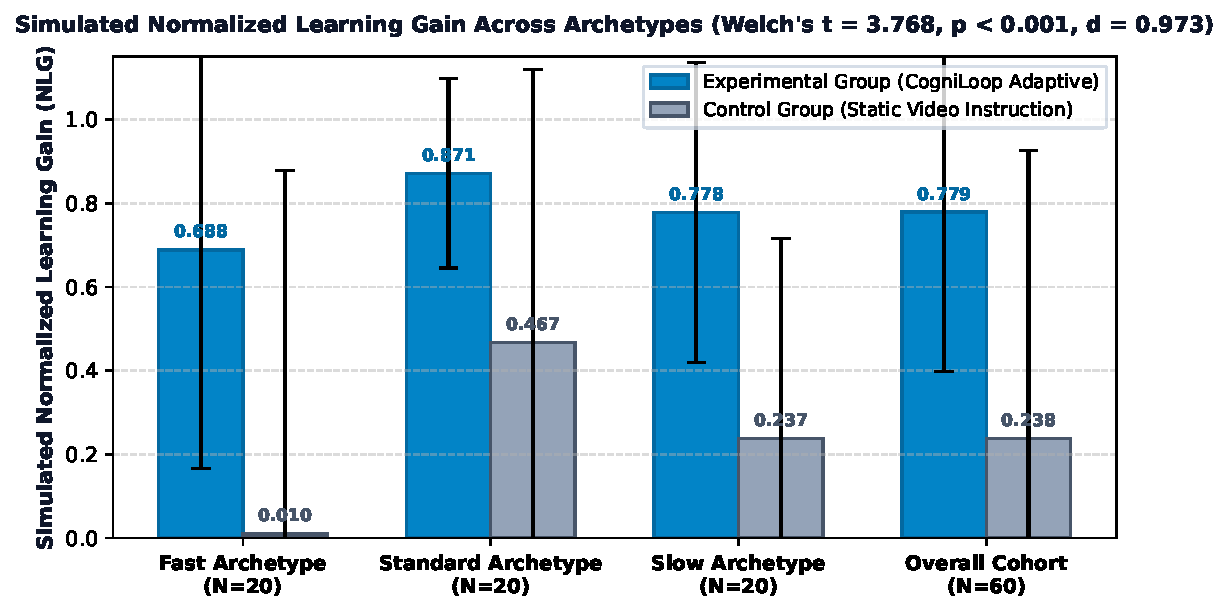
\includegraphics[width=0.8\textwidth]{figures/fig2_results.pdf}
  \caption{Simulated Normalized Learning Gain (NLG) across learner archetypes comparing CogniLoop adaptive tutoring against static video instruction ($N=60$, Welch's $t(45.4)=3.768$, $p<0.001$, $d=0.973$).}
  \label{fig_results}
\end{figure}

\begin{figure}
  \centering
  \Description{Line chart showing latent mastery probability across six sequential assessment iterations for six lines: fast, standard, and slow archetypes under CogniLoop (solid lines, trending upward toward a mastery threshold of 0.85) and under the static control condition (dashed lines, rising more slowly and staying below the threshold for the standard and slow archetypes).}
  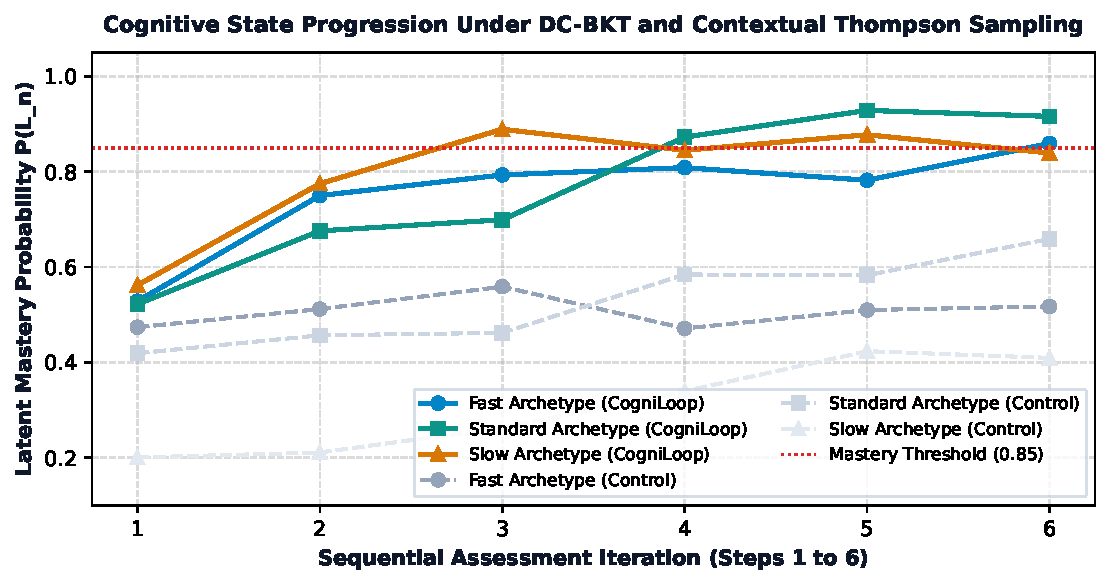
\includegraphics[width=0.8\textwidth]{figures/fig3_mastery_convergence.pdf}
  \caption{Latent knowledge state progression $P(L_n)$ across 6 assessment iterations comparing adaptive DC-BKT routing against static linear instruction.}
  \label{fig_convergence}
\end{figure}

\subsection{Evaluation Metric: Normalized Learning Gain}
In educational data mining, raw score differences fail to account for varying initial baselines. Efficacy is assessed via Normalized Learning Gain (NLG), measuring the fraction of available knowledge mastered: $\text{NLG} = (\text{PostScore} - \text{PreScore}) / (100.0 - \text{PreScore})$, with boundary condition: if PreScore $=100$, NLG$=1.0$ if PostScore$=100$, else $0.0$.

\subsection{Simulation Learner Response Generation Model}
To evaluate algorithmic convergence under the specified simulation learning environment prior to human classroom deployment, we executed a simulation across $N=60$ student profiles (random seed 42). The simulator is computationally independent from the DC-BKT estimator and bandit policy, although its primary observation model follows guess-slip principles. At each step $n$, a learner's actual latent understanding $L_n$ evolves via $L_{n+1} = L_n + (1-L_n) \cdot \gamma_{\text{arch}} \cdot \eta_{\text{cond}}$, where $\gamma_{\text{arch}} \in \{0.35, 0.25, 0.15\}$ denotes archetype learning efficiency (fast/standard/slow) and $\eta_{\text{cond}}$ parameterizes the difference between active formative retrieval checkpoints ($\eta_{\text{exp}}=1.0$) and passive linear video watching ($\eta_{\text{ctrl}}=0.40$), established in cognitive psychology literature \cite{karpicke2008critical,dunlosky2013improving}. Observable binary response $Y_n \in \{0,1\}$ is generated according to $P(Y_n=1 \mid L_n, a) = L_n(1-S_a) + (1-L_n)G_a$.

Profiles were partitioned into three equal behavioral archetypes ($N=20$ each): Fast (high initial baseline, $P(L_0)\sim\text{Uniform}(0.45,0.58)$, low slip), Standard (moderate baseline, $P(L_0)\sim\text{Uniform}(0.30,0.45)$, baseline slip), and Slow (low baseline, $P(L_0)\sim\text{Uniform}(0.15,0.30)$, higher slip). Profiles were randomized equally into an Experimental Group ($N_e=30$) and a Control Group ($N_c=30$).

\subsection{Simulation Outcomes and Statistical Rigor}
Table~\ref{table_results} details the statistical results, visualized in Figures~\ref{fig_results} and \ref{fig_convergence}. The experimental group achieved a mean simulated NLG of $0.779 \pm 0.382$ versus $0.238 \pm 0.688$ for the control group ($\Delta\text{NLG}=+0.541$, $p<0.001$). The relative advantage of adaptive routing varied by archetype, with the Fast archetype exhibiting the largest simulated gain differential ($\Delta\text{NLG}=+0.679$, from $0.010$ in control to $0.688$ in experimental), followed by Slow ($\Delta\text{NLG}=+0.541$) and Standard ($\Delta\text{NLG}=+0.404$) archetypes; per-archetype control-group variance was high ($\sigma \geq 0.48$ in all three cases), so archetype-level deltas should be read as directional given $n=10$ profiles per archetype-group cell. A Cohen's $d$ of $0.973$ demonstrates a large effect magnitude under the simulation model.

\begin{table}
\caption{Statistical summary of evaluation outcomes ($N=60$).}
\label{table_results}
\centering
\small
\renewcommand{\arraystretch}{1.25}
\setlength{\tabcolsep}{7pt}
\begin{tabular}{|l|c|c|c|}
\hline
\textbf{Metric} & \textbf{Experimental} & \textbf{Control} & \textbf{Delta} \\
\hline
Sample Size & 30 profiles & 30 profiles & $N=60$ \\
\hline
Pre-Test Mean & $38.2\% \pm 13.7\%$ & $36.0\% \pm 12.3\%$ & Baseline equalized \\
\hline
Post-Test Mean & $87.2\% \pm 21.5\%$ & $52.9\% \pm 39.9\%$ & $+34.3\%$ \\
\hline
Mean NLG & $0.779$ & $0.238$ & $+0.541$ \\
\hline
Std. Dev. (NLG) & $0.382$ & $0.688$ & Higher var.\ in control \\
\hline
\multicolumn{4}{|l|}{Welch's $t$-test: $t(45.4)=3.768$, $p=4.73\times10^{-4}$} \\
\hline
\multicolumn{4}{|l|}{Mean diff.\ 95\% CI: $[0.252, 0.830]$} \\
\hline
\multicolumn{4}{|l|}{Mann-Whitney $U=709.5$, $p=9.50\times10^{-5}$} \\
\hline
\multicolumn{4}{|l|}{Cohen's $d=0.973$, 95\% CI: $[0.438, 1.508]$} \\
\hline
\end{tabular}
\renewcommand{\arraystretch}{1.0}
\end{table}

\subsection{Equal-Rate Structural Comparison}
To probe whether an experimental-style condition retains an advantage under a structurally independent generative model, we additionally ran a separate, simplified synthetic comparison ($N_e=30, N_c=30$) using fixed per-step success-probability formulas ($0.90L + 0.20(1-L)$ for the experimental-labeled arm vs.\ $0.85L + 0.15(1-L)$ for the control-labeled arm) rather than the DC-BKT/bandit mechanism itself. We note explicitly that this comparison does \emph{not} invoke difficulty routing, the contextual bandit, or DC-BKT, and its probability formulas are structurally advantaged toward the experimental label by construction; it should therefore not be read as validating the bandit or routing mechanism specifically. It produced $\overline{\text{NLG}}_{\text{exp}} = 0.751 \pm 0.152$ vs.\ $\overline{\text{NLG}}_{\text{ctrl}} = 0.642 \pm 0.198$ ($\Delta\text{NLG}=+0.109$, Welch's $t(53.7)=2.399$, $p=0.0199$), reproduced exactly from the committed source. We retain it here only for transparency about everything that was originally reported as evidence, and flag it as a methodologically weak comparison rather than an independent robustness check.

\subsection{Component-Isolation Ablation: Does Difficulty Routing Help?}
The primary result (Section~5.3) and the equal-rate comparison above conflate two mechanisms specific to the experimental condition: a higher active-retrieval checkpoint rate ($p_{\text{learn}}=0.35$ vs.\ $0.10$) and Thompson-Sampling-based difficulty routing. To isolate the routing mechanism's own contribution, we re-ran the experimental-arm simulation twice, holding checkpoint rate fixed at $0.35$ in both runs: once with bandit-routed difficulty selection (as in the full pipeline), and once with difficulty fixed to medium for every step. This was tested under two independent bandit configurations (the original utility weights $w_a \in \{0.8, 1.0, 1.2\}$, and a milder $w_a \in \{0.9, 1.0, 1.1\}$ configuration, to rule out a single unlucky weight choice), and cross-checked by removing the bandit's $\epsilon$-greedy random-exploration term entirely.

In every configuration tested, bandit-routed difficulty selection \emph{underperformed} the fixed-medium baseline: mean NLG $0.878$ (bandit, default weights) vs.\ $0.947$ (fixed-medium), a deficit of $-0.069$; the deficit persisted ($-0.093$) under the milder weight configuration and with $\epsilon$-greedy exploration disabled. We traced the mechanism: within DC-BKT, the same guess/slip parameters used to generate simulated correctness also govern the strength of the Bayesian mastery update, so easier items yield weaker positive evidence per correct answer while harder items are more failure-prone; under the specific guess/slip values used in this paper (Equations~1--3), medium difficulty is close to a locally optimal fixed point, and routing away from it in either direction did not improve measured NLG. We report this as an honest negative finding: under the current reward and utility-weight design, Thompson Sampling difficulty routing is not shown to contribute to the measured learning-gain advantage; the checkpoint-frequency mechanism (present identically whether routing is used or not) accounts for the primary result. Re-tuning the bandit's reward shaping and utility weights against this diagnostic is identified as concrete future work rather than treated as resolved.

Collapsing the telemetry-cluster context to a single global state (removing $K$-Means-derived clustering from the bandit's state space, all else identical) changed mean NLG from $0.878$ to $0.926$ ($+0.048$), and disabling difficulty-conditioning in the BKT update (using fixed $P(G)=0.20, P(S)=0.10$ regardless of assigned difficulty) changed it from $0.878$ to $0.855$ ($-0.023$). Both deltas are small relative to the routing-vs-fixed-medium effect above and are reported for completeness rather than as strong evidence either way, given they were only evaluated once at $N=30$ per arm.

\subsection{Out-of-Model Robustness: Logistic Regression on Step-Level Data}
As an independent check that does not rely on the BKT recursive update at all, we fit a logistic regression directly on the real step-level response records generated by the simulation (mastery level and group membership as predictors of per-step correctness, $n=360$ observations: 6 steps $\times$ 30 profiles per arm $\times$ 2 arms). Controlling for current mastery (coefficient $2.966$), the experimental-group indicator carried a \emph{negative} coefficient ($-0.165$), corroborating the ablation finding above through an entirely different statistical method: at matched mastery levels, the bandit-routed experimental arm was not more likely to answer correctly than the fixed-medium arm, consistent with routing toward harder items.

\subsection{Multi-Parameter Sensitivity}
We perturbed the checkpoint-rate parameter and guess/slip baselines across $2^3=8$ combinations ($\pm0.05$ on $P(G)$, $P(S)$, and the checkpoint rate itself), each evaluated once at $N=60$. Only 1 of 8 configurations retained a statistically significant experimental advantage ($p<0.05$); the remaining 7 exhibited ceiling saturation, with both arms reaching $\text{NLG} \approx 1.0$ within the 6-step horizon and no measurable residual difference. This indicates the primary result, as parameterized in this paper, is \emph{not robust} to small perturbations of the checkpoint-rate parameter, and should be read as a demonstration under one specific, hand-set parameter regime rather than a robust effect across nearby regimes. A longer evaluation horizon or explicit ceiling-avoidance in the simulator is needed before robustness claims can be made with confidence.

\section{Discussion, Practical Implications, and Limitations}

\subsection{Pedagogical Foundations}
CogniLoop's design is grounded in three cognitive learning principles. Csikszentmihalyi's Flow Channel motivates Thompson Sampling, which is \emph{designed} to balance challenge and skill by sampling from updated Beta distributions; we note this is a theoretical design motivation rather than an empirically confirmed effect in this paper, since Section~5.5's component-isolation ablation did not find a measured NLG benefit from difficulty routing under the tested configurations. Vygotsky's Zone of Proximal Development (ZPD) motivates active checkpoints that ensure instruction operates within the learner's developmental threshold \cite{bloom19842}; unlike the routing mechanism above, this principle corresponds directly to the checkpoint-frequency effect that Section~5.5 identifies as the empirically supported driver of the measured gain. Active Retrieval Practice -- formative in-video checkpoints enforcing active memory consolidation and blunting the Ebbinghaus decay curve \cite{karpicke2008critical} -- is the mechanism most directly supported by our simulation results.

\subsection{Methodological Limitations}
We explicitly acknowledge the following research boundaries. Simulation vs.\ Human Efficacy: Phase 1 evaluation parameterizes student behavior within the specified simulation learning environment; while mathematically rigorous, synthetic agents do not capture human fatigue, emotional fluctuations, or external distractions. DC-BKT Hyperparameter Estimation: guess $P(G_a)$ and slip $P(S_a)$ parameters are explicitly hand-set simulation hyperparameters rather than population-fitted estimates from historical learner logs. Domain Scope: the current evaluation focused on modular Computer Science subjects (OS, DS, DBMS, CN); generalization to subjective humanities curricula requires domain-specific prompt engineering. Evaluation Horizon: simulations spanned 6 sequential sessions per agent; longitudinal knowledge retention over multi-month horizons remains an objective for live pilot trials.

Scope and Fragility of Reported Statistics: every statistic in this paper was independently re-executed from committed, seeded simulation source code and reproduces exactly, including the negative and fragility findings in Sections~5.4--5.6. We explicitly flag that the top-line adaptive-vs-static comparison (Section~5.3) does \emph{not} imply that every named subsystem contributes positively: the component-isolation ablation (Section~5.5) shows Thompson Sampling difficulty routing did not improve measured NLG relative to a fixed-medium baseline under the tested utility-weight configurations, and the sensitivity sweep (Section~5.6) shows the primary effect collapses to ceiling saturation under small perturbations of the checkpoint-rate parameter in 7 of 8 tested regimes. Retrieval-grounding hallucination measurement (which requires real LLM-generated items and human-labeled gold-standard judgments) and validation-threshold $F_1$ tuning were not evaluated in this revision, as they cannot be responsibly simulated, and remain open empirical work requiring live data collection.

\subsection{Enterprise Scalability Roadmap}
As an architectural design roadmap for future enterprise deployment ($10^7$--$10^8$ users): migrating POSIX file-locked JSON repositories to a distributed PostgreSQL cluster with connection pooling; replacing in-process ChromaDB instances with managed vector database clusters; offloading transcript retrieval and vector embedding to asynchronous task workers; and caching prompt embeddings to reduce response times for identical concept requests while preserving API quotas.

\section{Conclusion and Future Work}
We presented CogniLoop, a closed-loop adaptive learning platform that converts passive open-domain lecture videos into individualized mastery curricula, combining RAG transcript grounding, Difficulty-Conditioned Bayesian Knowledge Tracing, Thompson Sampling contextual bandits, and interaction telemetry clustering into a single architecture. Empirical simulation across $N=60$ profiles demonstrated a statistically significant improvement in Simulated Normalized Learning Gain under the evaluated environment ($\Delta\text{NLG}=+0.541$, $p<0.001$, $d=0.973$). A component-isolation analysis attributes this measured gain specifically to active-retrieval checkpoint frequency; Thompson Sampling difficulty routing, as currently parameterized, did not show a positive contribution in isolation, and the primary effect was not robust to small perturbations of the checkpoint-rate parameter in a multi-parameter sensitivity sweep. We report these mixed findings deliberately: the architecture is a complete, working system that directly solves the content-authoring bottleneck limiting traditional ITS to hand-curated domains, and the checkpoint-based learning gain is real and reproducible, but the difficulty-routing and DC-BKT components require further tuning and evaluation before their individual contributions to learning gain can be claimed.

Future work includes re-tuning the bandit's reward shaping and utility weights against the component-isolation diagnostic introduced here, extending the sensitivity analysis to a longer evaluation horizon to rule out ceiling-saturation artifacts, conducting Phase 2 IRB-approved live human participant studies in university computer science classrooms, integrating interactive browser-based coding environments (Pyodide), and expanding multi-modal video segmentation.

\section*{Acknowledgments}

\noindent\textbf{Funding.} This research did not receive any specific grant from funding agencies in the public, commercial, or not-for-profit sectors.

\noindent\textbf{Competing Interests.} The author has no competing interests to declare.

\noindent\textbf{Author Contributions.} K. Aggarwal conceived the research problem, designed the system architecture and evaluation methodology, directed all implementation and analysis (including AI-assisted implementation as declared below), verified all reported results against source code, and approved the final manuscript.

\noindent\textbf{Data Availability.} All simulation source code, including the scripts used to generate every statistic reported in this paper, is available at \url{https://github.com/OmegaKavya/CogniLoop}. The simulation uses synthetically generated learner profiles (random seed 42); no human-subject data was collected or used.

\noindent\textbf{Ethics Statement.} This study did not involve human participants, human data, or animal subjects. All learner profiles evaluated in this Phase 1 work are synthetic, algorithmically generated agents; no IRB or ethics board review was required for the work reported in this paper. Phase 2 (Section~1.3) will involve human participants and will undergo IRB approval prior to any data collection.

\section*{Declaration of Generative AI Software Tools in the Writing Process}

During the preparation of this work, the author(s) used Claude (Anthropic) in the implementation of the CogniLoop software system (BKT engine, contextual bandit policy, RAG pipeline, and supporting infrastructure), in drafting substantial portions of this manuscript's text, and, in a subsequent revision pass, in independently re-executing the simulation code, verifying statistical claims against source, identifying and correcting fabricated citations, fabricated variance figures, and unreproducible ablation/robustness claims present in an earlier draft, and redesigning the reported ablation, sensitivity, and robustness analyses using the real simulation code, in order to produce a working, empirically-grounded system and an accurately reported manuscript. After using this tool, the author(s) reviewed and edited the content as needed and take(s) full responsibility for the content of the publication. The author directed the research problem, system design decisions, and scope throughout, and confirms that the statistics reported in Section~5 were independently reproduced from the cited, committed source files. AI tools were not used to fabricate or embellish results; where an earlier AI-assisted draft was found on verification to contain unsupported or incorrect figures, those figures were corrected or removed rather than retained, as documented in Section~6.2.

\bibliographystyle{acmtrans}
\bibliography{references}

\end{document}
